\documentclass[tikz,border=10pt]{standalone}
% Coordinates: X=(px-263.7)*s, Y=(258.7-py)*s, s=0.017621 (longest side 8 cm)
\begin{document}
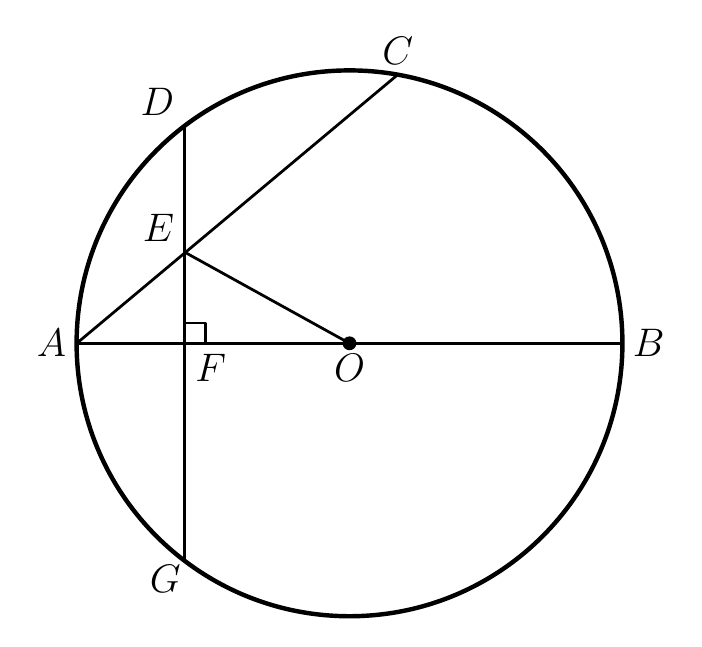
\begin{tikzpicture}[line join=round, line width=1.0pt,
  lab/.style={font=\fontsize{14}{16.8}\selectfont}]

% Named points (geometry unchanged)
\coordinate (O) at (0,0);
\coordinate (A) at (-3.464,0);
\coordinate (B) at (3.465,0);
\coordinate (F) at (-2.092,-0.005);
\coordinate (D) at (-2.092,2.764);
\coordinate (G) at (-2.092,-2.764);
\coordinate (E) at (-2.092,1.157);
\coordinate (C) at (0.612,3.411);

% Circle (radius unchanged, heavier stroke 1.6pt than the chords)
\draw[line width=1.6pt] (O) circle (3.466);

% Diameter AB, vertical DG, chord CA, segment OE (1.0pt from global style)
\draw (A) -- (B);
\draw (D) -- (G);
\draw (C) -- (A);
\draw (O) -- (E);

% Centre dot at O (enlarged to match original)
\fill (O) circle (2.5pt);

% Right-angle mark at F (side 15 px = 0.264 units)
\draw (-1.828,-0.005) -- (-1.828,0.259) -- (-2.092,0.259);

% Labels
\node[lab, left] at (A) {$A$};     % left of A, at baseline height
\node[lab, right] at (B) {$B$};    % right of B, at baseline height
\node[lab, above] at (C) {$C$};
\node[lab, above left] at (D) {$D$};
\node[lab, above left] at (E) {$E$};
\node[lab, anchor=north east, inner sep=1pt] at (G) {$G$}; % just below-left of G
\node[lab, below right] at (F) {$F$};
\node[lab, below] at (O) {$O$};
\end{tikzpicture}
\end{document}